\chapter{Aplikacja demonstracyjna}
\label{c6:c6}

\section{Opis aplikacji wspomagającej zarządzanie magazynem}
	\subsection{Założenia, wymagania oraz ich realizacja}
		Aplikacja przygotowana jako część praktyczna pracy dyplomowej miała za zadanie
		zobrazować niektóre z funkcji, które powinien spełniać system wspomagający
		zarządzanie gospodarką magazynową. Podstawowym wymaganiem stało się więc
		dostarczenie aplikacji dostępnej z każdego miejsca, posiadającej dostęp
		do centralnej bazy danych oraz wspartej oprogramowaniem umożliwiającym
		zaprogramowanie podstawowych algorytmów. Aplikacja jest dostępna przez interfejs przeglądarki
		internetowej, co daje możliwość korzystania na dowolnej maszynie, bez konieczności
		instalacji skomplikowanego oprogramowania. 
	\subsection{Dostępna funkcjonalność aplikacji}
		Istniejąca funkcjonalność zapewnia:
		\begin{itemize}
			\item Dostęp do funkcji aplikacji jedynie dla osób upoważnionych
			\begin{itemize}
				\item aplikacja rozpoznaje czy użytkownik jest już zalogowany
				\item użytkownik może w każdej chwili zakończyć pracę
				\item użytkownik jest automatycznie wylogowywane po 30 minutach 
			\end{itemize}
			\item Rejestracja nowego przedsiębiorstwa oraz pojedynczego magazynu;
			\item Rejestracje dowolnej ilości stref wydzielonych w magazynie, a także organizowania
			stref w strukturę drzew. Takie rozwiązanie jest elastycznym podejściem, które
			pozwala na przenoszenie ładunków między różnymi strefami, jeśli istnieje taka możliwość, tj.
			gdy strefa C jest, nie koniecznie bezpośrednim, potomkiem strefy A.
			\item Rejestracja nowych klientów: \textbf{dostawców oraz odbiorców}, którzy traktowani są
			zgodnie ze swoją funkcją w misji przedsiębiorstwa, czyli dostawca odpowiedzialny jest
			jedynie za dostawy. Niewykluczona jest sytuacja, gdy ten sam klient, jest zarówno dostawcą, jak
			i odbiorcą. 
		\end{itemize}
	\subsection{Realizacja postulatów aplikacji WMS}
		Aplikacja realizuje postulaty funkcjonalności WMS w obszarach wspomagania gospodarki magazynowej,
		ewidencji towarów, podziału magazyny na logiczne jednostki oraz utrzymania informacji
		o wydaniach / przyjęciach produktów. Odpowiednio wydanie towaru implikuje zmniejszenie stanów
		magazynowych, a przyjęcie zmniejszenie oraz alokację w strefach odkładczych.
	\subsection{Aplikacja widziana oczami programisty}
		Aplikacja wspomagająca zarządzanie magazynem została zaprojektowana i zbudowana jako aplikacja
		dostępna przez przeglądarkę. W założeniu istniało przygotowanie programu, którego będzie można
		używać na dowolnej z przeglądarek, obecnie istniejących na rynku, dzięki zastosowaniu
		narzędzi zapewniających taką kompatybilność. Cały program korzysta z architektury
		\textbf{klient - serwer - baza danych}, z silnikiem naciskiem położonym na funkcjonalność
		serwera. Część kliencka została zaprojektowana na wzór aplikacji desktop\footnote{
			\textbf{Aplikacja desktop} - aplikacja, którą można uruchomić na komputerach klasy PC,
			nie wymaga przeglądarki jako środowiska pracy, tylko odpowiednio przygotowane
			środowiska uruchomieniowe na docelowej platformie		
		} oraz zaimplementowana, w całości, przy użyciu kompletnego i zwartego framework'a\footnote{
			\textbf{Framework} - jest to całościowy zestaw bibliotek, narzędzi, a także zasad i wytycznych
			ułatwiających w znacznym sposób przygotowanie gotowej aplikacji		
		} JavaScript'owego \footnote{
			\textbf{JavaScript} - język wspierający idee programowania obiektowego i prototypowego, mający
			szerokie zastosowanie jako narzędzie wspierające wprowadzanie dynamiki do stron
			internetowych. 		
		}.
	\subsection{Architektura klient - serwer - baza danych oraz Model - Widok - Kontroler}
		\paragraph{Baza danych} jest warstwą danych dla projektu. Oparta o wolny i otwarty \footnote{
			Dostępny na licencji \href{http://www.gnu.org/licenses/old-licenses/gpl-2.0.html}{GPLv2}
		}
			serwer \textbf{MySQL}. Było to rozwiązanie podyktowane szerokim użyciem tego silnika w 
			na wielu serwisach, które umożliwiają hosting strong, czyniąc warstwę modelu danych możliwą
			do ponownego wykorzystania, bez konieczności, często problematycznego, migrowania danych do
			nowego silnika. \\
			Warto w tym miejscu wspomnieć o kolejnym narzędziu, które mimo, że działa na poziomie serwera, 
			odpowiada za dostarczenie odpowiedniej abstrakcji dla warstwy modelu danych i ułatwienia
			operacji nań. Wspomnianym narzędziem jest ogólnodostępne i otwarto źródłowy projekt Hibernate. 
			Konfiguracja jest oparta na co najmniej jednym pliku, tak jak na załączniku \ref{ca:hibernatecfg},
			który jest bezwzględnie wymagany. Niemniej można dodatkowo dodać wiele plików, również XML, z których
			każdy będzie opisem translacji danej klasy na odpowiadającą jej tabelę w systemie bazy danych. 
		\paragraph{Serwer} został napisany w całości w języku Java i oparty o kontener aplikacji webowych 
			\textbf{Tomcat}\footnote{
				\textbf{Apache Tomcat} - serwer aplikacji internetowych, którego główną częścią jest interakcja
				ze specjalnymi klasami znanymi jako \textit{servlety}, umożliwiających korzystanie z funkcjonalności
				jaką oferuje serwer przez standardowy protokół \textit{HTTP} i żądania \textit{CRUD}		
			}, a sama podstawową zasadą przy jego tworzeniu było oparcie centralny punkt wejściowy - fasadę, która dawała
			dostęp do całej funkcjonalności aplikacji przez zwarty interfejs, decydujący o wyborze konkretnego rozwiązania.
			\begin{table}[H]
				\begin{tabular}[c]{l*{2}{c}}
					Żądanie HTTP	& 	wartość zmiennej typu CRUD	\\
					\hline
					POST			&	CREATE						\\
					PUT				& 	UPDATE						\\
					DELETE			&	DELETE						\\
					GET				& 	READ						\\
				\end{tabular}
				\label{c6:tab:CRUD_matches}
				\caption[Żądania HTTP a typ wyliczeniowy CRUD]{Odpowiednie wartości typu wyliczeniowego \textit{CRUD}, a żądania HTTP}
			\end{table}
			Parametr typu \textbf{CRUD} przyjmuje jedną z 4 wartości:
			\textit{Create, Read, Update, Delete} zależnie od metody żądania HTTP, która go wywoła. Jest to najprostsza rzecz
			do ustalenia, ale prawdopodobnie jedna z najważniejszych. Znając jej wartość algorytm jest w stanie wywołać
			odpowiednie metody odpowiedzialne za obsługę zgłoszenia. Przykładowo, sytuacją oczekiwaną na żądania 
			\textit{GET} byłoby wystosowanie zgłoszenia do warstwy modelu danych, aby ta zwróciła zbiór wartości odpowiadających
			warunkom, jakie serwer odebrał od aplikacji klienckiej. 
			\begin{listing}[H]
				\inputminted[
					linenos=true,
					fontsize=\tiny,
					firstline=57, 
					lastline=75,
		            numbersep=15pt
				]{java}{../application/src/main/java/org/kornicameister/wms/server/servlet/WMSDataAgent.java}	
				\label{c6:listing:WMSDataAgent}
				\caption[WMSDataAgent - \textbf{processRequest}]{\textit{WMSDataAgent-processRequest} - 
				metoda rozdzielająca zadania na podstawie adresu oraz metody CRUD}
			\end{listing}
			\begin{listing}[H]
				\inputminted[
					linenos=true,
					fontsize=\tiny,
					firstline=32, 
					lastline=45,
		            numbersep=15pt
				]{java}{../application/src/main/java/org/kornicameister/wms/server/extractor/RDExtractor.java}	
				\label{c6:listing:WMSDataAgent}
				\caption[RDExtractor - \textbf{parse}]{\textit{RDExtractor-parse} - metoda parsująca żądania HTTP i zwracające 
				potrzebne opcje jako obiekt}
			\end{listing}
		\paragraph{Klient} jest warstwą reprezentują funkcjonalność serwera. Część ta dostępna jest przez praktycznie
		dowolną przeglądarkę internetową, więc działa jako tak zwana \emph{aplikacja internetowa}. Bardzo
		dużą zaletą takiego rozwiązania jest możliwość uruchomienia aplikacji na dowolnym urządzeniu klasy PC z zainstalowaną
		odpowiednią przeglądarką. Jako inne zalety można z pewnością wymienić: 
		\begin{itemize}
			\item większe możliwości rozbudowy, napraw i aktualizacji;
			\item aktualizacje dokonywane są w sposób transparentny dla użytkownika.
		\end{itemize}
		Ponadto praktycznym skutkiem było uzyskanie dostępu dla wszystkich żądań HTTP, które stanowią podstawę
		komunikacji między urządzeniami, a człowiekiem w dobie Internetu, jaka dzisiaj obowiązuje.
		\subparagraph{AJAX oraz REST} są wyznacznikami, które stały się głównym powodem wykorzystania
		framework'a ExtJS w wersji 4.1.3. AJAX jest technologią, która pozwala na wykonywania asynchronicznych
		zapytań pod wskazany adres i uaktualnianie stron internetowych bez konieczności ich przeładowania. 
		Z drugiej strony REST wprowadził dużo przejrzystości, potrzebnej przy budowanie tak rozbudowanej aplikacji,
		przy budowaniu adresów zapytań i ich obsłudze. W obecnej formie, zapytania różnią się, ta poziomie
		wskazania jaki rodzaj encji z bazy danych, klient chce obsłużyć. W efekcie, konfiguracja modeli ExtJS
		sprowadzała się do następujących 2 linijek:
		\begin{listing}[H]
			\inputminted[
				linenos=true,
				fontsize=\tiny,
				firstline=94, 
				lastline=97,
	            numbersep=10pt
			]{java}{../application/src/main/webapp/resources/app/model/entity/Unit.js}	
			\label{c6:listing:Unit.js}
			\caption[Unit.js - \textbf{model danych}]{\textit{Unit.js} - konfiguracja proxy
			modelu danych odpowiadającego podejściu REST}
		\end{listing} 
\section{Diagramy, zrzuty ekranowe oraz funkcje}
	\subsection{Logowanie do aplikacji przy pierwszym uruchomieniu}
		\begin{figure}[H]
			\centering
			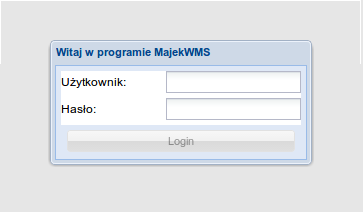
\includegraphics[width=0.99\textwidth]{images/app/login}
			\caption[Aplikacja - Logowanie do programu]{Zrzut ekranu pokazują aplikację w stanie tuż po uruchomieniu}
			\label{c7:fig:app:login}
		\end{figure}
		Aplikacja wspiera identyfikacje oraz autoryzacje użytkownik, jeszcze przed uruchomieniem programu. Praktycznie
		na każdym kroku, system sprawdza, czy użytkownik jest wciąż zalogowany, czy też nie. W drugim wypadku
		wystosowywane jest okno, takie jak na rysunku \label{c7:fig:app::login}. Mechanizm logowania został oparty
		o własne rozwiązanie zaimplementowane po stronie serwera, a wymagające podanie jedynie hasła oraz 
		nazwy użytkownika.\\ Można to łatwo zmienić, ponieważ operacja autoryzacji została wyodrębniona
		do samodzielnej \textbf{klasy servlet}. Korzyścią tego, a zarazem wytłumaczeniem prostoty rozszerzenia
		operacji autentyfikacji, jest zawsze występująca operacja:
		\begin{listing}[H]
			\inputminted[
				linenos=true,
				fontsize=\tiny,
				firstline=46, 
				lastline=97,
	            numbersep=10pt
			]{java}{../application/src/main/java/org/kornicameister/wms/server/servlet/WMSAuthAgent.java}	
			\label{c6:listing:WMSAuthAgent}
			\caption[WMSAuthAgent - \textbf{doPost}]{\textit{WMSAuthAgent-doPost} - metoda parsująca żądania POST, dokonująca
			autentyfikacji użytkownika na podstawie przekazanego loginu i hasła}
		\end{listing}
		W tym momencie uzyskujemy praktyczne wykorzystanie wzorca projektowego, znanego jako \textbf{fasada} lub bardziej
		w tym miejscu adekwatnego \textbf{mostu}. W oby wypadkach chodzi o dostarczenie zwartego i raczej 
		niezmiennego \textbf{API} - interfejsu programistycznego, gdzie tutaj, ten termin odnosi się
		do niezmiennej postaci funkcji obsługujących konkretne żądania HTTP.
		Istotnym więc jest jedynie aby wartość zwracana do klienta, była
		z nim kompatybilna i aplikacja kliencka była w stanie poprawnie ją odczytać, podczas gdy warstwa
		implementacji, dzięki której uzyskujemy pożądaną funkcjonalność,
		może zostać zmieniona w sposób transparenty dla części klienta. \\
		Ostatecznie aplikacja wymaga jednorazowego podania danych identyfikujących użytkownika oraz
		jest ona w stanie zapamiętać tę informację pomiędzy odświeżeniami aplikacji, jednocześnie
		dając możliwość zakończenia korzystania z programu w dowolnym momencie, poprzez operację
		wylogowania.
		
	\subsection{Zarządzanie strukturą magazynu}
		\begin{figure}[H]
			\centering
			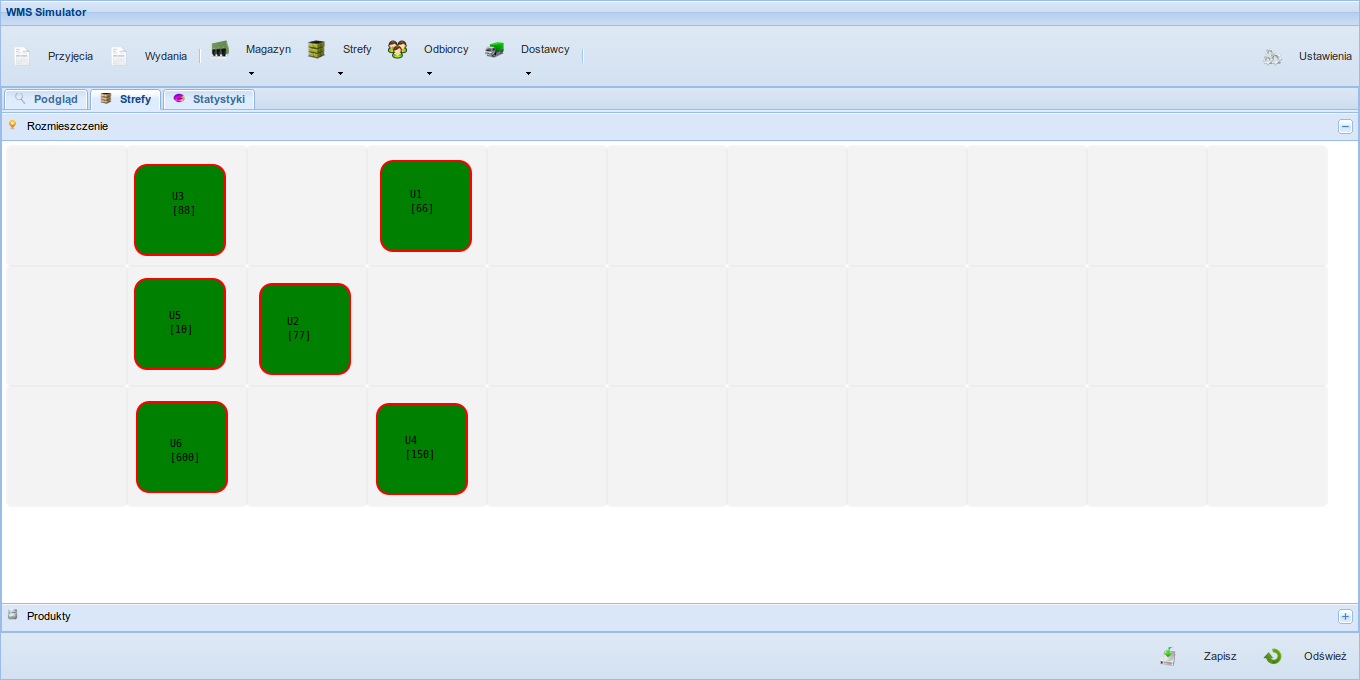
\includegraphics[width=0.99\textwidth]{images/app/unit_preview}
			\caption[Aplikacja - Zarządzania strukturą magazynu]{Zrzut ekranu z widokiem na strukturę magazynu}
			\label{c7:fig:app:unit_preview}
		\end{figure}
		
	\subsection{Zarządzanie klientami - dodawanie, usuwaniu, edycja oraz podgląd}
		\begin{figure}[h]
			\centering
			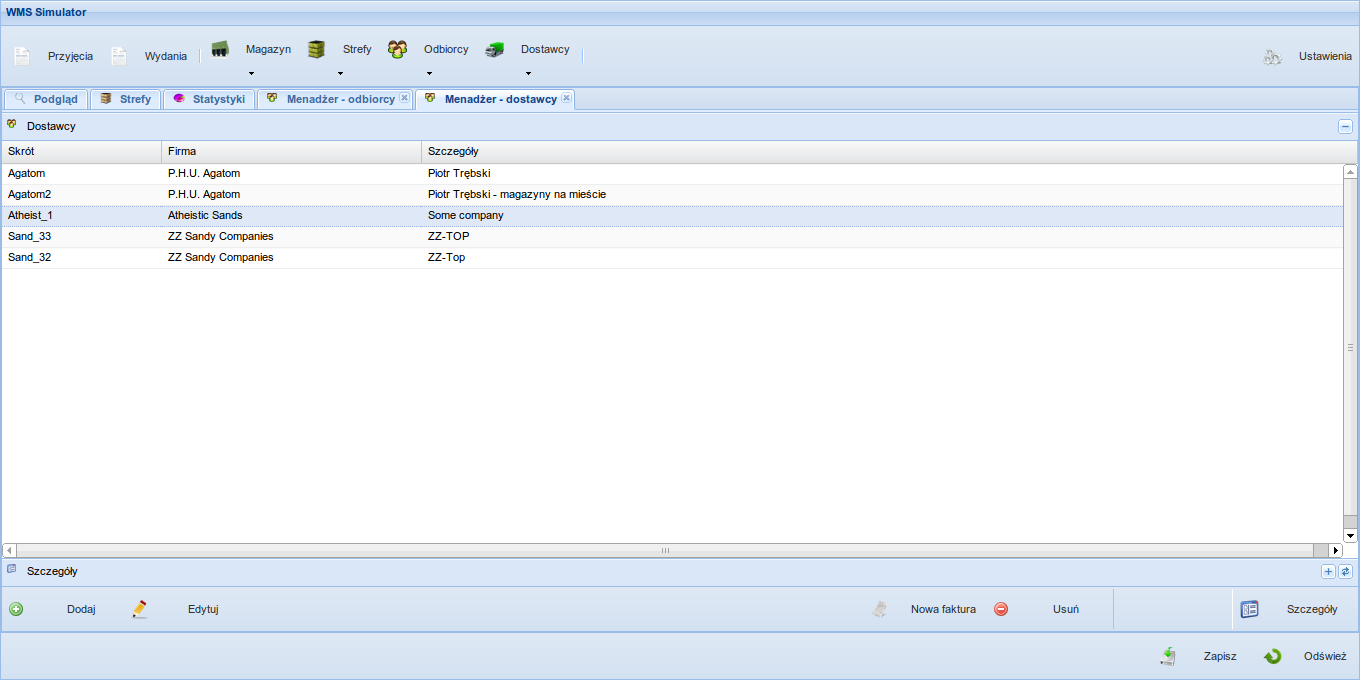
\includegraphics[width=0.99\textwidth]{images/app/supplier_preview}
			\caption[Aplikacja - Dostęp do danych klientów]{Zrzut ekranu z widokiem na dostępnych dostawców}
			\label{c7:fig:app:supplier_preview}
		\end{figure}
		\begin{figure}[h]
			\centering
			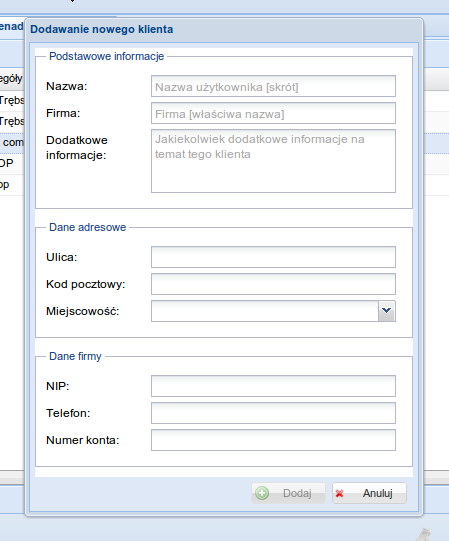
\includegraphics[width=0.6\textwidth]{images/app/new_receipient_dialog}
			\caption[Aplikacja - Dodawania nowego klienta - odbiorcy]{Zrzut ekranu z widokiem na okno dialogowe dla tworzenia nowego odbiorcy}
			\label{c7:fig:app:new_receipient_dialog}
		\end{figure}
		
		\paragraph{Zarządzanie klientami} odbywa się z wydzielonych zakładek, z których jedna przeznaczona jest
		dla \textbf{dostawców}, a druga dla \textbf{odbiorców}. Podejście takie pozwoliło na zobrazowanie problemu,
		kiedy jedna instytucja istnieje w systemie jednocześnie jako dostawca i klient. Podstawowa funkcjonalność tego
		modułu obejmuje:
		\begin{itemize}
			\item dodawanie oraz usuwanie danych o klientach (rysunki: \ref{c7:fig:app:supplier_preview} oraz \ref{c7:fig:app:new_receipient_dialog});
			\item pogląd (uproszczony) listy wszystkich dostawców oraz odbiorców (rysunek \ref{c7:fig:app:supplier_preview});
			\item podgląd na dokumenty wydań/przyjęć dla wybranej pozycji.
		\end{itemize}
		Podzielenie widoku na listy zarejestrowanych klientów zwiększa czytelność, a także daje możliwość edycji dowolnej pozycji,
		niezależnie od tego czy jest to kontrahent, czy też jedna z przypisanych doń pozycji w dokumentach.		
		
	\subsection{Wydanie, przyjęcia oraz ewidencja produktów}
		\begin{figure}[h]
			\centering
			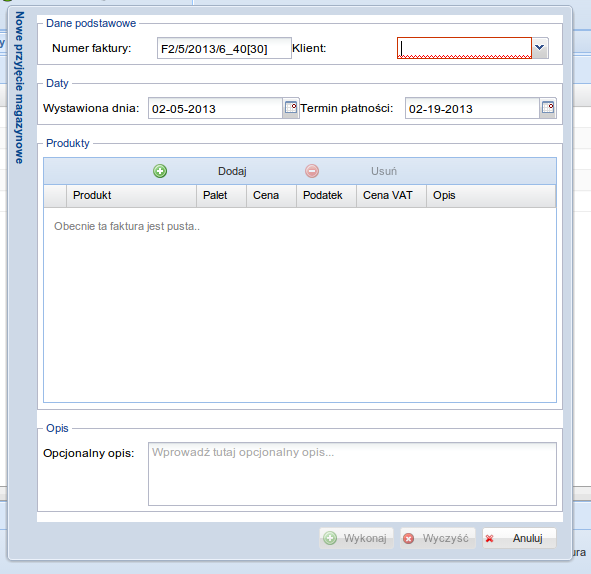
\includegraphics[width=0.99\textwidth]{images/app/new_supply_preview}
			\caption[Aplikacja - Dodanie nowego dokumentu wydania]{Zrzut ekranu z widokiem na kreator nowego wydania magazynowego}
			\label{c7:fig:app:new_supply_preview}
		\end{figure}
		
		\paragraph{Operacja wydania} jest operacją, która może zostać wykonana jedynie dla tych kontrahentów, którzy są odbiorcami
		produktów, składowanych w magazynie. Zgodnie z rysunkiem \textbf{\ref{c7:fig:app:new_supply_preview}} każdy z dokumentów
		magazynowych składa się z następujących pozycji:
		\begin{itemize}
			\item numeru faktury, nadawanego arbitralnie aby uniknąć pomyłek oraz zapewnić, że każda z faktur jest 
			jednoznacznie identyfikowana przez klucz, jakim jest numer faktury;
			\item klienta (w tym wypadku odbiorcy), który jest odbiorcą\footnote{Jedynie tacy kontrahenci będący odbiorcami mogą
			zostać wybrani i są dostępni na liście rozwijanej};
			\item daty wystawienia oraz odbioru, które muszą różnić się o co najmniej \textbf{14 dni};
			\item listy produktów\footnote{Produkty pobierane są z bazy danych. Wynika z tego, że zarówno dla operacji przyjęcia, jak i wydania
			produkt musi być obecny w bazie};
			\item dodatkowych uwag, przeznaczonych dla odbiorcy odnośnie danego dokumentu oraz jego zawartości.
		\end{itemize}
		Zatwierdzenie takiego dokumentu powoduje, że dla danego odbiorcy zapisana zostaje informacja o utworzonym dla niego
		wydania magazynowym,a stany magazynowe zostają zmniejszone, zgodnie z informacją podaną na fakturze. 
		
		\paragraph{Operacja przyjęcia} jest operacją prawie identyczną różniącą się w następujących miejscach:
		\begin{itemize}
			\item klientami, są jedynie ci kontrahenci, którzy w systemie istnieją jako dostawcy i tylko tacy są widoczni
			w liście rozwijanej;
			\item zatwierdzenie dokumentu przyjęcia magazynowego, powoduje uruchomienie odpowiedniego algorytmu alokującego
			\footnote{Algorytmy alokacji można znaleźć w załączniku \ref{ca:allocationAlgorithms}}
			produkty i zwiększenie stanów magazynowych dla każdego z produktów, tak jak to podano na fakturze.
		\end{itemize}
		
		\paragraph{Ewidencja produktów} jest kolejną funkcjonalnością, potrzebną w systemie WMS.
		Moduł ten pozwala poznać strukturę magazynu i to, jak zostały rozłożone produkty w systemie.
		Każdy z pozycji opisana jest przez następujące atrybuty: 
		\begin{itemize}
			\item nazwę;
			\item ilość aktualnie przechowywanych palet w danej strefie;
			\item cenę jednostkową;
			\item naliczony podatek;
			\item opcjonalny opis.
		\end{itemize}
		\begin{figure}[h]
			\centering
			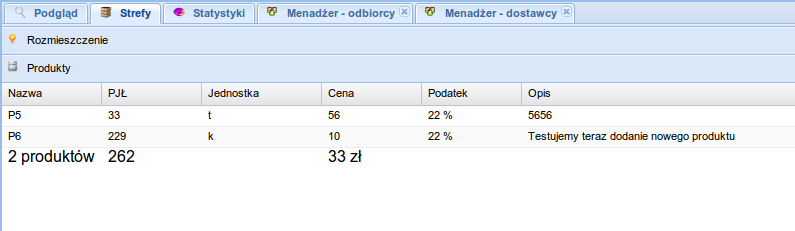
\includegraphics[width=0.8\textwidth]{images/app/unit_products_preview}
			\caption[Aplikacja - Ewidencja towarów w poszczególnych strefach]{Zrzut ekranu z widokiem listy produktów w wybranej strefie}
			\label{c7:fig:app:unit_products_preview}
		\end{figure}